\documentclass[10pt]{article}
\usepackage[letterpaper,margin=0.85in]{geometry}
\usepackage{amsmath,amssymb,booktabs,array,tabularx,graphicx,xcolor,enumitem,fancyhdr}
\usepackage{fontspec}
\setmainfont{DejaVu Serif}
\setsansfont{DejaVu Sans}
\usepackage[colorlinks=true,linkcolor=blue!45!black,urlcolor=blue!45!black,citecolor=blue!45!black]{hyperref}
\definecolor{ink}{HTML}{17334D}
\definecolor{accent}{HTML}{167D8D}
\pagestyle{fancy}\fancyhf{}
\fancyhead[L]{\small\sffamily ARC White-Box Estimation · Phase 2}
\fancyhead[R]{\small\sffamily Submission 336809}
\fancyfoot[L]{\footnotesize Final technical writeup · 18 October 2026}
\fancyfoot[R]{\thepage}
\setlength{\headheight}{15pt}
\setlength{\parindent}{0pt}\setlength{\parskip}{6pt}
\setlist{nosep,leftmargin=1.4em}
\setlength{\emergencystretch}{2em}
\newcommand{\E}{\mathbb E}
\newcommand{\Cov}{\operatorname{Cov}}
\newcommand{\diag}{\operatorname{diag}}
\newcommand{\ReLU}{\operatorname{ReLU}}
\newcommand{\clip}{\operatorname{clip}}
\newcommand{\code}[1]{\texttt{\small #1}}
\newcommand{\sectionpage}[1]{\clearpage\section{#1}}
\title{\vspace{-1.5em}\color{ink}\sffamily Covariance-defect correction and\newline transported mean innovations\newline for white-box MLP estimation}
\author{Tristan Miano\\\small AIcrowd: \texttt{tristan\_miano}}
\date{Phase 2 technical writeup · Submission \textbf{336809}\\
\small Algorithm ALG058-V001 · 18 October 2026}

\begin{document}
\maketitle\thispagestyle{fancy}
\begin{abstract}
We describe the estimator submitted as \textbf{336809}, which attained a public
budget-adjusted final-layer mean squared error of
\(2.97110640613\times10^{-9}\), with raw error
\(1.94467643766\times10^{-8}\). It builds on the published factored cumulant
engine of 504aldo and LordProcciuto. Our additions are a fitted, analytically
motivated covariance-defect dictionary inside the physical recurrence, and
small learned local mean innovations propagated through a separate linear
response recurrence. The final model averages two fixed innovation sources,
preserving their separate feature normalizations in one batched evaluation.

On four exposed development networks, our complete adaptation reduces
adjusted error by \textbf{4.55\%} relative to the unmodified public engine under
the same current FLOP meter. The final mean-source addition also improves the
official score by \textbf{2.05\%} relative to our covariance-only entry. These
are different comparisons. The much larger 28.50\% improvement over our earlier
incumbent is predominantly associated with adopting the public cost engine;
we do not claim that improvement as our independent contribution. We document
training, resource measurements, unsuccessful alternatives, and the limits of
the evidence. Private final evaluation has not yet occurred.
\end{abstract}

\section{Problem and score}
For a fixed, bias-free, width-1024, depth-16 ReLU MLP with known weights,
\begin{equation}
 h_0=X\sim\mathcal N(0,I),\qquad h_\ell=\ReLU(W_\ell h_{\ell-1}),
 \qquad m_\ell=\E_X[h_\ell],
\end{equation}
the estimator returns all layer means; the scored error is on layer 16.
For network \(j\), with counted compute \(C_j\) and budget \(B=2^{41}\),
\begin{equation}\label{eq:score}
 s_j=\frac{\|\widehat m_{16,j}-m_{16,j}\|_2^2}{1024}
       \max\{0.1,C_j/B\},\qquad S=\frac1N\sum_j s_j.
\end{equation}
The score is the \emph{mean of per-network products}; multiplying mean error
by mean compute is generally incorrect. The challenge uses a separate fresh
private evaluation for final rankings~\cite{rules,update}.

\sectionpage{Published foundation and our changes}
Wu et al.~\cite{wu} develop cumulant and Hermite methods for propagating
activation distributions through random MLPs. Our submission belongs to that
family. It does not run Monte Carlo input samples at inference.

The direct implementation base is LordProcciuto's MIT-licensed
\texttt{e30\_a}, commit \texttt{3d038e9}, derived from 504aldo's MIT V29
engine~\cite{lord,aldo}. We retain its approximate mean/covariance propagation,
factored third-order history, regenerated fourth-order information, pruning,
fixed transported bases, matrix-product engineering, and existing fitted
87-feature mean correction. Those are credited prior work. The final archive
preserves both authors' MIT notices.

\begin{figure}[!ht]
\centering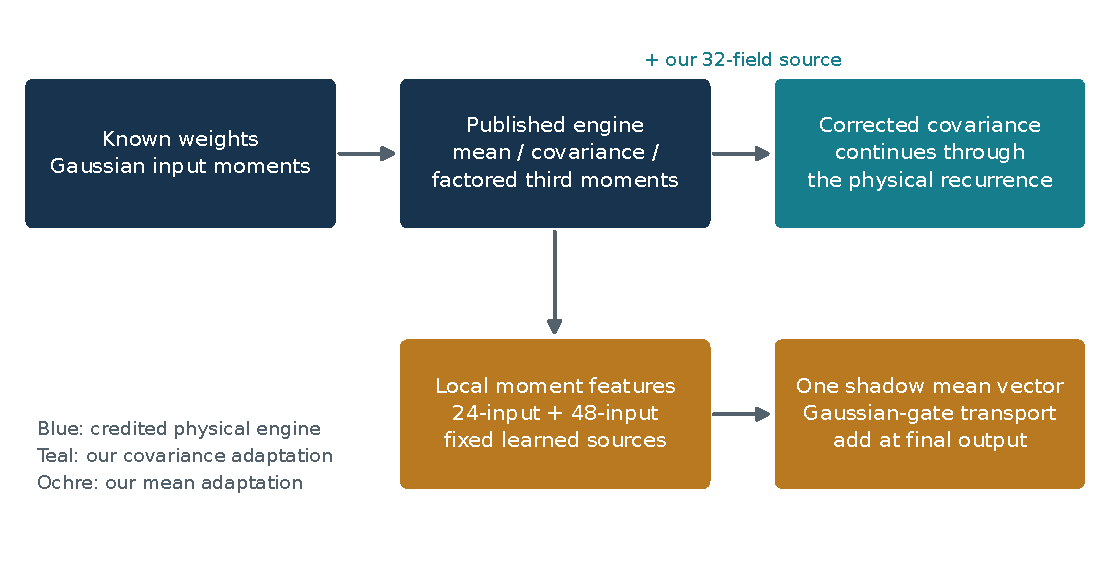
\includegraphics[width=\linewidth]{images/method.pdf}
\caption{The two additions act at different places. Our covariance source
changes the continuing physical state. The new mean-source vector follows
that trajectory but does not feed back into it.}
\end{figure}

\begin{tabularx}{\linewidth}{@{}p{.25\linewidth}X@{}}\toprule
Component & Contribution claimed in this report\\\midrule
Physical covariance & A 32-field defect dictionary, 96 fitted coefficients
across three layer groups, including marginal, mixed, and quadratic
third-cumulant shapes; an algebraic regrouping of its evaluation.\\
Mean innovation & A trace-informed local feature representation, training on
layerwise error innovations, and one transported response vector.\\
Final combination & Equal averaging of independently trained 24-input and
48-input source models, with their normalization and clipping preserved in a
single batched call.\\\bottomrule
\end{tabularx}

These are adaptations of established cumulant, response, and learned-closure
ideas. We make no claim to have invented cumulant propagation, Hermite
expansions, residual learning, or model averaging. The covariance dictionary
is mechanistically motivated; its coefficients and the mean-source functions
are learned. The submission is therefore not a parameter-free deduction from
the published equations.

\sectionpage{A covariance-defect source inside the recurrence}
At a preactivation, write mean \(\mu_i\), variance \(v_i=\sigma_i^2\),
off-diagonal covariance \(c_{ij}\), and \(\alpha_i=\mu_i/\sigma_i\).
Define the Gaussian-smoothed ReLU derivatives
\begin{equation}\label{eq:derivatives}
 f_i^{(0)}=\mu_i\Phi(\alpha_i)+\sigma_i\phi(\alpha_i),\quad
 f_i^{(1)}=\Phi(\alpha_i),\quad
 f_i^{(r)}=\frac{(-1)^{r-2}\operatorname{He}_{r-2}(\alpha_i)
 \phi(\alpha_i)}{\sigma_i^{r-1}}\quad(r\ge2).
\end{equation}
Here \(\phi,\Phi\) are the standard Gaussian density and CDF, and
\(\operatorname{He}_r\) are probabilists' Hermite polynomials. These are
derivatives of a Gaussian convolution, so no ordinary higher derivative of
the nonsmooth ReLU needs to be evaluated.

For jointly Gaussian coordinates, the off-diagonal covariance expansion is
\begin{equation}\label{eq:gauss}
 \Cov_G(f(Z_i),f(Z_j))=
 \sum_{r\ge1}\frac{c_{ij}^{r}}{r!}f_i^{(r)}f_j^{(r)}.
\end{equation}
A formal first-order marginal third-cumulant perturbation suggests fields
\begin{equation}\label{eq:s3}
 S^{(3)}_{r,ij}=\frac{c_{ij}^{r}}{6r!}
 \left[k_{3,i} f_i^{(r+3)}f_j^{(r)}+
       k_{3,j} f_j^{(r+3)}f_i^{(r)}\right].
\end{equation}
Mixed third cumulants instead supply shapes beginning with
\(\tfrac12 T_{iij}f_i^{(2)}f_j^{(1)}+(i\leftrightarrow j)\).
Products of third cumulants supply additional quadratic shapes. The
dictionary also includes diagonal variance sources and fourth-cumulant
terms; Appendix~\ref{app:dictionary} specifies all 32 fields.

These expressions motivate a \emph{defect dictionary}, not a list of proven
missing terms. The base already includes some of their effects. Adding each
textbook coefficient with unit strength would double-count contributions.
Instead, the actual postactivation covariance is changed by
\begin{equation}\label{eq:covupdate}
 C_\ell^+\leftarrow C_{\ell,\mathrm{base}}^+
       +\sum_{a=1}^{32}\beta_{g(\ell),a}S_a,\qquad
 g(\ell)=\min\{\lfloor(\ell-1)/5\rfloor,2\}.
\end{equation}
The correction is used after layers 1--15; no covariance is needed after the
final mean readout. Its diagonal is also added to the stored variance vector.
This state subsequently affects transport and nonlinear moment production.

\textbf{Fitting.} The 96 coefficients were fitted previously on 32 exposed
training networks using a Gaussian mean/covariance response model. The loss
combines normalized local mean innovations and terminal mean error, with
diagonal ridge regularization \(\lambda=10^{-3}\). The target trajectory then
included an earlier mean corrector. All 96 coefficients were transferred
unchanged to the newer public engine; they were not refitted for submission
336809. The response is an approximation to the derivative of the full
algorithm, so actual integrated evaluations, rather than the fit alone,
establish the reported gains.

\textbf{Evaluation cost.} Terms sharing a power of \(c_{ij}\) or a cumulant
slice are grouped. Sums of separable kernels become small products
\(A B^T\), reducing Python operations and repeated elementwise work. This is
an algebraic regrouping; floating-point evaluation order can change.

\sectionpage{Learning and transporting local mean innovations}
Let \(b_\ell\) be the base prediction along the covariance-corrected trajectory,
and let \(e_\ell=m_\ell-b_\ell\) be its training error. Set
\(J_\ell=\diag(\Phi(\alpha_\ell))W_\ell\). Our supervised target is
\begin{equation}\label{eq:innovation}
 u_\ell=e_\ell-J_\ell e_{\ell-1},\qquad \ell=2,\ldots,16.
\end{equation}
This separates locally generated error from error already carried through
the linearized mean map. For any chosen \(J_\ell\), the identity is exact if
the true errors are supplied; interpreting \(J_\ell\) as the response of the
full cumulant estimator is an approximation.

At inference, a source model predicts \(\widehat u_\ell\) from current
moments, and one shadow vector evolves as
\begin{equation}\label{eq:shadow}
 r_1=0,\qquad r_\ell=J_\ell r_{\ell-1}+\widehat u_\ell.
\end{equation}
The new vector does not change the physical mean, covariance, or cumulant
history. It is added at the last layer. In the exact code order the final
output is \([b_{16}^{\rm core}+r_{16}]_++d_{16}\), where \(d_{16}\) is the
public engine's separately restored contribution from pruned neurons. Earlier
returned layer means remain the physical predictions.

\textbf{Features.} The local source receives 24 features: normalized mean,
skewness and fourth cumulant; relative log variance; eight pairwise
correlation/cumulant summaries; three layer/global scalars; and nine signed
mean/trace projections. Appendix~\ref{app:features} gives their formulas.
The context source adds the within-layer neuron average of each local feature,
giving 48 inputs. At the final layer, the pair and trace features are set to
zero because the public engine omits those expensive final-layer slices.

For either input vector \(x_i\), a model is
\begin{align}
 z_i&=\clip((x_i-a)/s,-8,8),\nonumber\\
 \widehat u_{\ell,i}&=10^{-3}\sigma_i\phi(\alpha_i)
       \left[w_{h(\ell)}^T\tanh(H z_i+b)+d_{h(\ell)}\right].\label{eq:nn}
\end{align}
Each has 32 hidden units and four output heads, selected for layers
2--6, 7--11, 12--15, and 16. The prefactor provides activation units and
suppresses corrections far from the ReLU boundary. It does not prove that the
learned source equals an omitted cumulant term.

\textbf{The shipped combination.} The 24-input model was trained on 32
networks; the 48-input model was trained on 64, including those 32. The
submission uses their fixed equal average. No mixture weight was fitted.
Because the models have different means and scales, their overlapping
features are duplicated before normalization: 72 coordinates feed a
block-diagonal 64-unit hidden layer, with halved output weights. There are
2,632 independently learned neural parameters before this deterministic
combination, plus feature statistics. Batching preserves the mathematical
function, not bitwise equality to separate float32 evaluation. The recorded
four-head feature test found maximum absolute difference
\(7.15\times10^{-7}\) before the amplitude prefactor. Exact-byte replay was
checked separately for the shipped package.

\sectionpage{Measured performance and attribution}
The three recent entries were graded successfully on 17 October and their
scores were rechecked on 18 October. Table~\ref{tab:official} reports official
public results. Only \textbf{336809} is the submission associated with this
writeup; the other IDs are comparison evidence.

\begin{table}[h]\centering\small
\begin{tabular}{@{}llrr@{}}\toprule
Submission & Method & Raw MSE & Adjusted score\\\midrule
335391 & Earlier engine + covariance & \(2.01272\!\times\!10^{-8}\) & \(4.15562\!\times\!10^{-9}\)\\
336778 & Public e30 + our covariance & \(1.98938\!\times\!10^{-8}\) & \(3.03329\!\times\!10^{-9}\)\\
336785 & Above + trace source & \(1.95309\!\times\!10^{-8}\) & \(2.98282\!\times\!10^{-9}\)\\
\textbf{336809} & \textbf{Above + equal source average} & \(1.94468\!\times\!10^{-8}\) & \(2.97111\!\times\!10^{-9}\)\\\bottomrule
\end{tabular}
\caption{Official public grades. The older entry was evaluated before the
latest meter update; this historical sequence is not a controlled cost ablation.}
\label{tab:official}
\end{table}

The final score is 28.50\% below our earlier incumbent. Raw error falls only
3.38\%; the ratio of aggregate score/error ratios is 0.73998. That second
quantity is an error-weighted multiplier comparison, \emph{not} the mean FLOP
ratio. The main cost-engine improvements belong to the public authors.

To isolate the incremental effect of our adaptation, Table~\ref{tab:four}
uses the same four exposed development networks and the same current runtime
for every row. There is no official unmodified-base submission in this
controlled comparison.

\begin{table}[h]\centering\small
\begin{tabular}{@{}lrrrr@{}}\toprule
Method & Raw MSE & FLOPs & Adjusted & Reduction\\
 & \(10^{-8}\) & \(10^9\) & \(10^{-9}\) & vs public\\\midrule
Public e30 engine & 2.11094 & 336.173 & 3.22335 & ---\\
+ our covariance & 2.02488 & 338.069 & 3.10976 & 3.52\%\\
+ trace source & 2.00623 & 338.606 & 3.08614 & 4.26\%\\
+ equal source average & 1.99919 & 338.738 & 3.07676 & 4.55\%\\\bottomrule
\end{tabular}
\caption{Matched development ablation on rows 750, 976, 772, 795;
FlopScope 0.12.3 / WhestBench 0.16.2. These are adaptively reused development
inputs, not a fresh held-out test. FLOPs are unweighted means; adjusted scores
are computed per network before averaging.}\label{tab:four}
\end{table}

The physical covariance addition costs about 0.56\% extra arithmetic in this
comparison. The complete adaptation costs about 0.76\% more than the public
engine and reduces raw error by 5.29\%. Its adjusted benefit therefore survives
the measured compute charge.

The newer mean corrections also have a wider comparison: on 12 development
networks the trace source improves adjusted score by 2.23\% over covariance
alone, winning 11/12; officially the improvement is 1.66\%. The final equal
average improves another 0.170\% locally and 0.393\% officially. Combined, the
official mean-source gain over covariance alone is 2.05\%. This supports a
modest additional benefit, not a claim that the learned sources explain the
large historical score reduction.

\sectionpage{Training and strength of the evidence}
\textbf{Network-level splits.} The covariance and original trace source use
32 exposed public training networks. The context source uses those 32 plus
32 additional public training networks. Four folds hold out whole networks,
not individual neurons. Final assets use all networks in their stated
training sets. The 12 submission-facing development rows are disjoint from
those fitting rows, but were repeatedly used during the research campaign.
Our protected final local blind block was not used in this task or to choose
these submitted assets. Local errors use the organizer's reference means,
not independently known exact expectations; finite-reference error was not
subtracted.

\textbf{Mean-source training.} Both models use 1,000 Adam updates with learning
rate 0.01, batches of 32,768 neuron/layer examples, gradient norm clipping at
5, and parameter-mean-square penalty \(10^{-4}\). The source-error loss is
normalized by the training RMS innovation at each layer, floored at
\(10^{-8}\). Feature standard deviations are floored at \(10^{-12}\).
Normalization and layer loss scales are computed from the training fold.
The output layer is initialized to zero; final-fit initialization and batch
generator seeds are 172018 and 172118. Training uses PyTorch offline;
inference uses fixed JSON assets and permitted FlopScope operations.

\begin{table}[h]\centering\small
\begin{tabular}{@{}llrr@{}}\toprule
Source & Response-model evaluation & Raw error ratio & Wins\\\midrule
Trace24 & Four folds, original 32 networks & 0.97486 & 26/32\\
Context48 & Four folds, expanded 64 networks & 0.96752 & 56/64\\
Frozen Trace24 & Additional 32 trajectories & 0.96352 & 30/32\\\bottomrule
\end{tabular}
\caption{Ratios to the covariance-only trajectory in the offline response
calculation. They are conditional/adaptive evidence, not integrated native
cross-validation or independent private-suite estimates.}
\end{table}

The covariance coefficients already depend on the original 32 networks, so
holding out a network for the source model does not make the entire pipeline
independent of that network. Architecture choices also used development
feedback. Offline response results can differ from a full estimator run,
especially when changing the physical state or its pruning decisions.

\begin{figure}[!ht]\centering
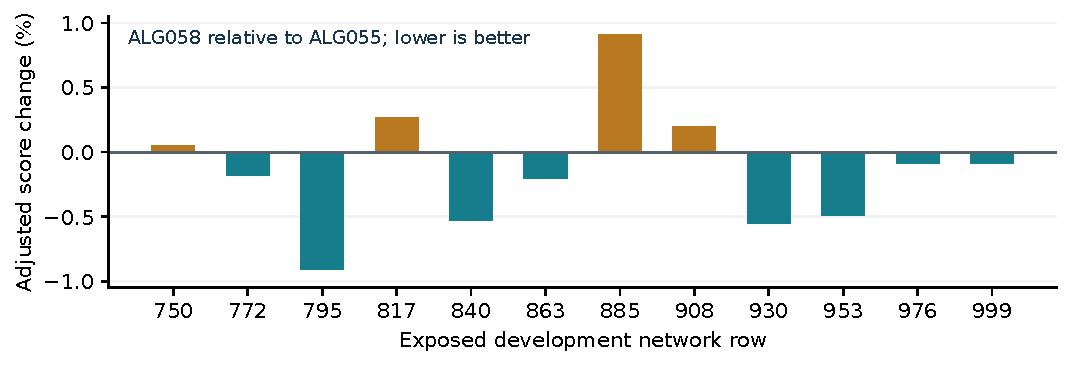
\includegraphics[width=\linewidth]{images/paired12.pdf}
\caption{The final combination wins 8/12 exposed development comparisons
against the simpler trace model. The plotted percentage is per network;
the pooled adjusted-score reduction is 0.170\%.}
\end{figure}

The archived bootstrap support for a lower pooled mean in this last comparison
is 0.893; its 90\% ratio interval is [0.99624, 1.00058]. Because these inputs
were adaptively reused, this is descriptive resampling support, not an 89.3\%
probability of winning the final private evaluation. The official public
improvement provides additional feedback, but that leaderboard also guided
development. We do not infer a confidence interval for the private rank.

\sectionpage{Failures, limitations, and resource behavior}
\textbf{Corrections are trajectory-dependent.} Transferring our older fitted
mean corrections directly to the cheaper public engine gave four-network
adjusted scores around \(3.40\)--\(3.53\times10^{-9}\), worse than the public
engine's \(3.22\times10^{-9}\). Refitting the local mean source on the new
covariance-corrected trajectory worked. Conversely, refitting all covariance
coefficients on the new trajectory did not improve the tested conditional
cross-validation. There is no general guarantee that a more recently fitted
or more flexible corrector is better.

\textbf{A promising small pilot can reverse.} A contextual source split
between physical mean feedback and the shadow vector improved a four-network
pilot by 1.08\% but lost by 0.53\% on the 12-network comparison. It was not
submitted. The 64-network context source alone was effectively tied with the
trace source on the larger comparison; the retained gain comes from their
combination. We did not establish why that averaging helps. Error
complementarity is a plausible interpretation, not an isolated mechanism.

\textbf{More moment information can cost too much.} Exploratory prototypes
using ARC's carried-fourth equations and a public scale-extraction
proposal~\cite{scale} showed roughly 15--20\% raw-error reductions on two
training networks. A literal rank-32 compression/transport implementation
projected about 51\% extra arithmetic, whereas its measured raw reduction
would tolerate only about 18\% extra compute above the score floor. This
combines research accuracy with separately metered kernels; it is neither an
integrated score nor a lower bound on the method family. These prototypes are
not part of submission 336809. They remain open research routes requiring
substantial cost reductions.

\textbf{Operational improvement mattered.} Evaluating the two source models
separately exceeded the 0.4-second residual-time cap on one local archive
case (0.401164 seconds). That version was not uploaded. Batching the unchanged
models produced the accepted version and passed the recorded full-shape
checks. Table~\ref{tab:resources} reports observed maxima, not guarantees for
every future network or host.

\begin{table}[h]\centering\small
\begin{tabular}{@{}lrr@{}}\toprule
Resource & Observed for ALG058-V001 & Limit\\\midrule
Counted FLOPs, per network & \(328.222\)--\(351.376\times10^9\) & \(2^{41}\)\\
Residual wall time, maximum & 0.387661 s & 0.4 s\\
Predict wall time, maximum & 44.285 s & 120 s\\
Setup time, maximum & 0.047888 s & 5 s\\
Process peak RSS & 6,086,852,608 bytes & \(2^{33}\) bytes\\\bottomrule
\end{tabular}
\caption{Preserved pilot and clean-archive qualification evidence under the
current local runtime. Twelve distinct full-size inputs plus repeated-input
checks; all recorded checks pass.}\label{tab:resources}
\end{table}

The package returns finite \(16\times1024\) predictions and has a separate
shape-generic smoke-test path inherited from the base. It does not establish
that the fitted corrections generalize to other widths, depths, activations,
or weight distributions. Resource failures and accuracy losses were recorded
separately throughout development.

\sectionpage{Reproducibility, provenance, and disclosure}
\textbf{Exact submitted artifact.} The report concerns submission
\textbf{336809}, ALG058-V001. Its accepted archive is identified by SHA-256:
\begin{quote}\small\ttfamily
2c28711f6d44709182886eb6e1535503af415\newline
ecd97721b46868b39f2ff0660db
\end{quote}
The two lines concatenate to one digest. The estimator and neural-asset
digests, source map, and training row lists are in Appendix~\ref{app:repro}.
The archive already held by AIcrowd contains the executable estimator,
fixed asset, metadata, README, and preserved licenses. A later documentary
clarification must not be confused with changing that accepted code.

Local qualification used Python 3.12.3, WhestBench 0.16.2, FlopScope and
FlopScope-server 0.12.3, and NumPy 2.2.6. The evaluator was updated to these
meter versions before the three recent submissions. The algorithm's numeric
inference operations use FlopScope; no runtime training, network access,
hidden grader information, or target lookup is used. Exposed challenge training
labels and weights remain in the research data store rather than in the
submitted estimator.

\textbf{Development.} Earlier work investigated sampling/variance reduction,
Gaussian and higher-cumulant closures, covariance response models, and learned
corrections. The retained implementation combines a published efficient
engine with the covariance fields developed in our earlier recurrence and
the two newer source models. It reflects both mathematical derivation and
empirical fitting. Most explored alternatives were not incorporated. The
report focuses on the accepted algorithm and the evidence needed to assess
its added value rather than presenting every research attempt as a finding.

\textbf{LLM assistance and author responsibility.} LLM coding agents performed
most of the code writing, mathematical exploration, experiment orchestration,
literature inspection, and report drafting. Substantial earlier work used
GPT-5.6 Sol; later work primarily used GPT-6 Astra at extra-high effort,
running locally through the ChatGPT Desktop application. A recorded
Ultra-effort trial used parallel sub-agents; smaller contributions came from
Fable and Opus sessions. Tristan Miano set objectives, directed the research
strategy, authorized tasks and submission attempts, and reviewed progress.
Claims of identities are supported by
the displayed algebra or recorded numerical checks; explanations of empirical
success that were not isolated experimentally are labeled as hypotheses.
The participant is responsible for the final submitted report.

\textbf{Scope of originality.} Public cumulant machinery, its fitted reference
tables, pruning, and core cost engineering are not ours. Our claim is the
specific covariance-defect adaptation, local-source construction, and their
measured incremental value in this estimator. We do not claim academic
priority for the general methods. The organizer's public-code clarification
requires substantial own changes; this report provides evidence for review
and does not claim advance eligibility approval~\cite{reuse}. The official
result is an improvement on our prior entries, not proof that this is the
best published estimator or a future prize winner.

\clearpage
\small
\begin{thebibliography}{9}\setlength{\itemsep}{2pt}
\bibitem{wu} W. Wu, V. Lecomte, M. Winer, G. Robinson, J. Hilton, and P. Christiano.
\emph{Estimating the expected output of wide random MLPs more efficiently than sampling}.
arXiv:2605.05179v2, 2026. \url{https://arxiv.org/abs/2605.05179v2}.
\bibitem{aldo} 504aldo. \emph{whest-p2-cumulant-k3}, V29. MIT-licensed public implementation.
\url{https://github.com/504aldo/whest-p2-cumulant-k3}.
\bibitem{lord} LordProcciuto. \emph{whestbench-lordprocciuto}, e30\_a and accompanying writeup.
MIT; commit \texttt{3d038e9f48a97671878ee7bbef02e193f128b61c}.
\url{https://github.com/siming767-creator/whestbench-lordprocciuto}.
\bibitem{rules} ARC / AIcrowd. \emph{Official challenge rules}, accessed 18 October 2026.
\url{https://www.aicrowd.com/challenges/arc-white-box-estimation-challenge-2026/challenge_rules}.
\bibitem{update} AIcrowd. \emph{Phase 2 update}, 17 October 2026.
\url{https://discourse.aicrowd.com/t/18251}.
\bibitem{reuse} AIcrowd. \emph{Eligibility of solutions built on another participant's MIT-licensed forum code},
5 October 2026. \url{https://discourse.aicrowd.com/t/18240}.
\bibitem{scale} il.miscusi. \emph{Removing the global scale mode makes a carried
fourth-cumulant core pay}, Phase 2 writeup for submission 336317,
15 October 2026. \url{https://discourse.aicrowd.com/t/18248}.
\end{thebibliography}
\normalsize
\clearpage\appendix
\section{The covariance dictionary}\label{app:dictionary}
This appendix specifies the unfused 32-field construction. The submitted code
evaluates its weighted sum in grouped kernels. For distinct \(i,j\), abbreviate
\(c=c_{ij}\), \(a=k_{3,i}\), \(b=k_{3,j}\), \(t=T_{iij}\),
\(u=T_{jji}\), \(q_i=k_{4,i}\), and \(\gamma_i=q_i/v_i^2\).
Write \(F_{pq}=f_i^{(p)}f_j^{(q)}\), with derivatives from
Eq.~\eqref{eq:derivatives}. \(K_{31,ij}\) and \(K_{22,ij}\) are the base's
available mixed fourth-cumulant approximations, not observed true cumulants.
In the code these are \code{wk431} and \code{wk4m}, respectively;
\(k_3,T,k_4\) use \code{D3}, \code{D21}, and \code{g4row}.
Each listed field has an independent coefficient in each of three layer bins.

\textbf{Six basic fields.} Let
\(V_i^G=(\mu_i^2+v_i)\Phi(\alpha_i)+\mu_i\sigma_i\phi(\alpha_i)
 -(f_i^{(0)})^2\). The first two fields are diagonal matrices with entries
\(V_i^G\) and \(V_i^G\gamma_i\). The four off-diagonal fields are
\begin{equation}
 \tfrac12 c F_{11}(\gamma_i+\gamma_j),\qquad
 \frac{c^r}{r!}F_{rr}\quad(r=2,3,4).
\end{equation}
All their unspecified diagonal entries are zero.

\textbf{Eight marginal fields.} Two diagonal fields are
\begin{equation}
 \frac{k_{3,i}}3[f_i^{(2)}-f_i^{(0)}f_i^{(3)}],\qquad
 \frac{k_{4,i}}{12}[f_i^{(3)}-f_i^{(0)}f_i^{(4)}].
\end{equation}
For \(r=1,2,3\), six off-diagonal fields are
\begin{equation}
 \frac{c^r}{6r!}(aF_{r+3,r}+bF_{r,r+3}),\qquad
 \frac{c^r}{24r!}(q_iF_{r+4,r}+q_jF_{r,r+4}).
\end{equation}

\textbf{Eight mixed/reference fields.} The first seven are
\begin{align}
 &\frac{c^r}{2r!}(tF_{r+2,r+1}+uF_{r+1,r+2}),&&r=0,1,2,\nonumber\\
 &\frac{K_{22,ij}c^r}{4}F_{r+2,r+2},&&r=0,1,\nonumber\\
 &\frac{c^r}{6}(K_{31,ij}F_{r+3,r+1}+K_{31,ji}F_{r+1,r+3}),&&r=0,1.
\end{align}
The eighth is \(C^+_{\rm base}-G_8\) off the diagonal, where
\(G_{8,ij}=\sum_{r=1}^{8}c^rF_{rr}/r!\). This allows a fitted correction to
the difference between the base pair closure and its order-eight Gaussian
reference. The unfused helper clips normalized correlation near \(\pm1\);
the shipped fused kernel evaluates the corresponding polynomial directly
from the carried covariance. Exact shipped code is the authority at numerical
boundaries.

\textbf{Ten quadratic third-cumulant fields.} The first two are
\begin{equation}
 \frac{c}{72}(a^2F_{71}+b^2F_{17}),\qquad \frac{cab}{36}F_{44}.
\end{equation}
For each \(r=0,1\), four more are
\begin{align}
 &\frac{c^r}{8}(t^2F_{r+4,r+2}+u^2F_{r+2,r+4}),\qquad
 \frac{c^r tu}{4}F_{r+3,r+3},\nonumber\\
 &\frac{c^r}{12}(atF_{r+5,r+1}+buF_{r+1,r+5}),\qquad
 \frac{c^r}{12}(btF_{r+2,r+4}+auF_{r+4,r+2}).
\end{align}
Their diagonals are zero. The formulas motivate signed residual shapes; they
do not assert that each missing term can be uniquely identified from fitted
coefficients. The 96 shipped values exactly match the preserved all-32-network
fit. They are included in the machine-readable evidence rather than rounded
into this report.

\clearpage
\section{Mean-source features and training objective}\label{app:features}
Define \(R_{ij}=c_{ij}/(\sigma_i\sigma_j)\),
\(P_{ij}=T_{iij}/(v_i\sigma_j)\), \(g_{3,i}=k_{3,i}/\sigma_i^3\),
\(g_{4,i}=k_{4,i}/v_i^2\), and
\(\tau_i=\sum_j T_{jji}+k_{3,i}\). Angle brackets denote a neuron average at
the current layer. Superscript \(\circ r\) means entrywise power.

\begin{tabularx}{\linewidth}{@{}p{.17\linewidth}X@{}}\toprule
Group & Features (in the implemented order)\\\midrule
Local (4) & \(\alpha_i,\ g_{3,i},\ g_{4,i},\ \log(v_i/\langle v\rangle)\).\\[3pt]
Pair (8) & \(\begin{aligned}
&\sum_jR_{ij}^2,\ \sum_jR_{ij}^3,\ \sum_jR_{ij}^4,\ \sum_jP_{ij}^2,\\
&\sum_jP_{ji}^2,\ \sum_jR_{ij}P_{ij},\ \sum_jR_{ij}P_{ji},\ (R^{\circ2}g_4)_i.
\end{aligned}\)\\[3pt]
Global (3) & \(\langle g_4\rangle,\ \langle g_3^2\rangle,\ (\ell-1)/15\).\\[3pt]
Trace/signed (9) & \(\begin{aligned}
&\sum_jP_{ij},\ \sum_jP_{ji},\ (R\alpha)_i,\ (P\alpha)_i,\ (P^T\alpha)_i,\\
&((R\circ P)\alpha)_i,\ ((R\circ P^T)\alpha)_i,\ \tau_i/(\sigma_i\langle v\rangle),\\
&\langle\tau\mu\rangle/(\langle\mu^2\rangle\langle v\rangle+10^{-30}).
\end{aligned}\)\\\bottomrule
\end{tabularx}

The 48-input model appends 24 neuron-averaged features. Its statistics are
computed from the features as represented by the public engine, including
pruning conventions. The final layer uses zero pair and signed/trace blocks.
The 24-input model and 48-input model have different normalization statistics;
duplicating local coordinates in the batch preserves both sets of clipping
boundaries. Replacing them with a common normalizer would be a different model.

For source training, with training-fold layer RMS \(s_\ell\), the minibatch
objective is
\begin{equation}
 \mathcal L(\theta)=\operatorname{mean}_{(j,\ell,i)\in\mathcal B}
 \left[\frac{\widehat u_{j\ell i}(\theta)-u_{j\ell i}}{s_\ell}\right]^2
 +10^{-4}\frac{\|\theta\|_2^2}{\#\theta}.
\end{equation}
The 24-input final fit has 932 learned parameters; the 48-input model has
1,700. The merged 64-unit representation contains structural zeros and a
combined output bias, so counting every stored array element as an independent
learned parameter would overstate the fitted degrees of freedom.

The innovation identity check in the research code starts from the observed
first-layer error and reconstructs the final observed error to numerical
precision. Deployment starts its additional response at zero and predicts
the later innovations. Thus that identity check validates the construction of
training targets; it does not prove the deployed response is exact or that
the first-layer error is identically zero.

For covariance fitting, let \(R_{j\ell}\beta\) denote the approximate mean
response and \(B_{j\ell}\beta=R_{j\ell}\beta-J_{j\ell}R_{j,\ell-1}\beta\).
The linear fitting system combines
\begin{equation}
 \operatorname{mean}_{j,\ell,i}
 \frac{(B_{j\ell}\beta-u_{j\ell})_i^2}{s_\ell^2}
 +\operatorname{mean}_{j,i}
 \frac{(R_{j,16}\beta-e_{j,16})_i^2}{s_{16,\rm end}^2}
 +10^{-3}\beta^T\diag(G)\beta,
\end{equation}
where \(G\) is the normalized design Gram matrix, with a \(10^{-30}\)
floor on its diagonal in the implementation. The coefficients were selected
from the local-plus-terminal objective; terminal-only fitting was a diagnostic
alternative. The later full-state evaluation is not identical to this linear
response model.

\clearpage
\section{Artifact identity and evidence map}\label{app:repro}
The accepted estimator and fixed neural asset have the following SHA-256
digests (join the wrapped lines):
\begin{quote}\small\ttfamily
estimator.py:\newline
6c295943161d1365afa042948770e451091d\newline
6fe16706ee7728505ece62b4ab44\medskip\newline
nn\_asset.json:\newline
bd824f7c1a7e4d1392e0b8507931e973237e\newline
b3ca02cabc9a07b66970d2c8e856
\end{quote}
The accepted archive, source files, current working copies, and stored
qualification hashes were compared on 18 October 2026; all matched. This was
an identity audit using existing evidence, not another numerical qualification
campaign. The live API still reported submission 336809 as successfully graded
with the scores shown in Table~\ref{tab:official}.

\begin{tabularx}{\linewidth}{@{}p{.24\linewidth}X@{}}\toprule
Claim / component & Repository evidence or code location\\\midrule
Accepted implementation & \path{submissions/phase2_alg058_v001/estimator.py};
mean-source call around lines 3287--3311; covariance update around 3540;
fused helper \code{\_fused\_cov\_delta}.\\
Covariance fit & \path{experiments/theory/t170/fit_quadratic.py} and
\path{experiments/theory/t170/P27_FIT/RESULT.json}.\\
Source models & \path{experiments/theory/t172/train_source.py},
\path{train_expanded_source.py}, and \path{build_anchor_merged.py}
(last two in the same directory).\\
Matched public-base comparison & \path{experiments/theory/t172/runs/},
probes P02\_e30, P09\_fused\_cov, P19\_new\_trace, P82\_anchor\_merged.\\
Official and qualification records & \path{experiments/theory/t172/candidates/},
ALG054-V000, ALG055-V000, ALG058-V001.\\
Report evidence index & \path{experiments/finalization/t173/WRITEUP_EVIDENCE.json},
\path{PACKAGE_IDENTITY_AUDIT.json}, and \path{CURRENT_GRADES.json}
(all in that directory).\\\bottomrule
\end{tabularx}

The curated public repository is
\url{https://github.com/TristanMiano/arc-whitebox-estimation-2026}.
It includes exact accepted packages, the final report sources, selected
research evidence, individual algorithm writeups, and a model/workflow and
timing audit. Some historical paths refer to the larger retained local
workspace. Raw challenge weights, labels, caches, and private repository
history are not republished. The AIcrowd submission ID resolves the accepted
executable package.

\textbf{Training rows.} Labels come from the organizer's
\path{aicrowd/arc-whestbench-public-2026} Full dataset; the original layer-label
manifest pins revision \texttt{ce926b7d1ced65faa668c01b94a43f8c4f43783d}.
The original 32 exposed dataset positions were
\begin{quote}\small
0, 16, 32, 48, 64, 80, 97, 113, 129, 145, 161, 177, 193, 209, 225, 241,
258, 274, 290, 306, 322, 338, 354, 370, 386, 402, 419, 435, 451, 467, 483, 499.
\end{quote}
The additional 32 were
\begin{quote}\small
8, 23, 39, 55, 70, 86, 102, 117, 133, 148, 164, 180, 195, 211, 227, 242,
259, 273, 289, 305, 320, 336, 352, 367, 383, 398, 414, 430, 445, 461, 477, 492.
\end{quote}
The submission-facing development order was 750, 976, 772, 795, 817, 840,
863, 885, 908, 930, 953, 999. These are dataset row identifiers, not seeds or
network identifiers used by the submitted inference algorithm.

\end{document}
